%%%%%%%%%%%%%%%%%%%%%%%%%%%%%%%%%%%%%%%%%
% Masters/Doctoral Thesis 
% LaTeX Template
% Version 2.1 (2/9/15)
%
% This template has been downloaded from:
% http://www.LaTeXTemplates.com
%
% Version 2.0 major modifications by:
% Vel (vel@latextemplates.com)
%
% Original authors:
% Steven Gunn  (http://users.ecs.soton.ac.uk/srg/softwaretools/document/templates/)
% Sunil Patel (http://www.sunilpatel.co.uk/thesis-template/)
%
% License:
% CC BY-NC-SA 3.0 (http://creativecommons.org/licenses/by-nc-sa/3.0/)
%
%%%%%%%%%%%%%%%%%%%%%%%%%%%%%%%%%%%%%%%%%

%----------------------------------------------------------------------------------------
%	PACKAGES AND OTHER DOCUMENT CONFIGURATIONS
%----------------------------------------------------------------------------------------

\documentclass[
11pt, % The default document font size, options: 10pt, 11pt, 12pt
%oneside, % Two side (alternating margins) for binding by default, uncomment to switch to one side
english, % ngerman for German
singlespacing, % Single line spacing, alternatives: onehalfspacing or doublespacing
%draft, % Uncomment to enable draft mode (no pictures, no links, overfull hboxes indicated)
%nolistspacing, % If the document is onehalfspacing or doublespacing, uncomment this to set spacing in lists to single
%liststotoc, % Uncomment to add the list of figures/tables/etc to the table of contents
%toctotoc, % Uncomment to add the main table of contents to the table of contents
%parskip, % Uncomment to add space between paragraphs
]{MastersDoctoralThesis} % The class file specifying the document structure

\usepackage[utf8]{inputenc} % Required for inputting international characters
\usepackage[T1]{fontenc} % Output font encoding for international characters

\usepackage{palatino} % Use the Palatino font by default
\usepackage{amssymb}
\usepackage[many]{tcolorbox}
\usepackage{amsthm}
\usepackage{algorithm}
\usepackage{algpseudocode}
\usepackage{listings}
\usepackage{tikz}
\usepackage{caption}
\usepackage{subcaption}
\usetikzlibrary{automata,positioning}

\usepackage{tkz-graph}
\GraphInit[vstyle = Shade]
\tikzset{
  LabelStyle/.style = { rectangle, rounded corners, draw,
                        minimum width = 2em, fill = yellow!50,
                        text = red, font = \bfseries },
  VertexStyle/.append style = { inner sep=5pt,
                                font = \Large\bfseries},
  EdgeStyle/.append style = {->, bend left} }
\thispagestyle{empty}




\newtheorem{theorem}{Theorem}[section]
\newtheorem{corollary}{Corollary}[theorem]
\newtheorem{lemma}[theorem]{Lemma}
\theoremstyle{definition}
\newtheorem{definition}{Definition}[section]

\usepackage[backend=bibtex,style=authoryear,natbib=true]{biblatex} % User the bibtex backend with the authoryear citation style (which resembles APA)

\addbibresource{example.bib} % The filename of the bibliography

\usepackage[autostyle=true]{csquotes} % Required to generate language-dependent quotes in the bibliography


\usepackage{xcolor,fancybox}
\usepackage[many]{tcolorbox}
\usepackage{lipsum}
\usepackage{varwidth}
\newtcolorbox{mybox}[2][]{enhanced,
attach boxed title to top left={xshift=1cm,yshift=-2mm},
fonttitle=\bfseries,varwidth boxed title=0.7\linewidth,
colbacktitle=green!45!white,coltitle=green!10!black,colframe=green!50!black,
interior style={top color=yellow!10!white,bottom color=green!10!white},
boxed title style={enhanced,boxrule=0.75mm,colframe=white,
borderline={0.1mm}{0mm}{green!50!black},
borderline={0.1mm}{0.75mm}{green!50!black},
interior style={top color=green!10!white,bottom color=green!10!white,
middle color=green!50!white},
drop fuzzy shadow},
overlay unbroken and first ={
    \node[fill=red, text=white, rounded corners] at (frame.east) {$\clubsuit$};
    },
title={#2},#1}
\newcommand{\pyobject}[1]{\ovalbox{\color{red}{\texttt{#1}}}}




%----------------------------------------------------------------------------------------
%	THESIS INFORMATION
%----------------------------------------------------------------------------------------

\thesistitle{Fast Projection on Birkhoff polytope} % Your thesis title, this is used in the title and abstract, print it elsewhere with \ttitle
\supervisor{Dr. Rolf \textsc{Bardeli}} % Your supervisor's name, this is used in the title page, print it elsewhere with \supname
\examiner{} % Your examiner's name, this is not currently used anywhere in the template, print it elsewhere with \examname
\degree{Masters of Science} % Your degree name, this is used in the title page and abstract, print it elsewhere with \degreename
\author{Mohammad \textsc{Saifullah}} % Your name, this is used in the title page and abstract, print it elsewhere with \authorname
\addresses{} % Your address, this is not currently used anywhere in the template, print it elsewhere with \addressname

\subject{Media Informatics} % Your subject area, this is not currently used anywhere in the template, print it elsewhere with \subjectname
\keywords{} % Keywords for your thesis, this is not currently used anywhere in the template, print it elsewhere with \keywordnames
\university{\href{http://www.rwth-aachen.de}{RWTH Aachen University}} % Your university's name and URL, this is used in the title page and abstract, print it elsewhere with \univname
\department{\href{http://department.university.com}{Fraunhofer IAIS}} % Your department's name and URL, this is used in the title page and abstract, print it elsewhere with \deptname
\group{\href{http://researchgroup.university.com}{Research Group Name}} % Your research group's name and URL, this is used in the title page, print it elsewhere with \groupname
\faculty{\href{http://faculty.university.com}{Faculty Name}} % Your faculty's name and URL, this is used in the title page and abstract, print it elsewhere with \facname

\hypersetup{pdftitle=\ttitle} % Set the PDF's title to your title
\hypersetup{pdfauthor=\authorname} % Set the PDF's author to your name
\hypersetup{pdfkeywords=\keywordnames} % Set the PDF's keywords to your keywords

\begin{document}

\frontmatter % Use roman page numbering style (i, ii, iii, iv...) for the pre-content pages

\pagestyle{plain} % Default to the plain heading style until the thesis style is called for the body content

%----------------------------------------------------------------------------------------
%	TITLE PAGE
%----------------------------------------------------------------------------------------

\begin{titlepage}
\begin{center}

\textsc{\LARGE \univname}\\[1.5cm] % University name
\textsc{\Large Masters Thesis}\\[0.5cm] % Thesis type

\HRule \\[0.4cm] % Horizontal line
{\huge \bfseries \ttitle}\\[0.4cm] % Thesis title
\HRule \\[1.5cm] % Horizontal line
 
\begin{minipage}{0.4\textwidth}
\begin{flushleft} \large
\emph{Author:}\\
\href{http://www.johnsmith.com}{\authorname} % Author name - remove the \href bracket to remove the link
\end{flushleft}
\end{minipage}
\begin{minipage}{0.4\textwidth}
\begin{flushright} \large
\emph{Supervisor:} \\
\href{http://www.jamessmith.com}{\supname} % Supervisor name - remove the \href bracket to remove the link  
\end{flushright}
\end{minipage}\\[3cm]
 
\large \textit{A thesis submitted in fulfilment of the requirements\\ for the degree of \degreename}\\[0.3cm] % University requirement text
\textit{in the}\\[0.4cm]
\groupname\\\deptname\\[2cm] % Research group name and department name
 
{\large \today}\\[4cm] % Date
%\includegraphics{Logo} % University/department logo - uncomment to place it
 
\vfill
\end{center}
\end{titlepage}

%----------------------------------------------------------------------------------------
%	DECLARATION PAGE
%----------------------------------------------------------------------------------------

\begin{declaration}
\addchaptertocentry{\authorshipname}

\noindent I, \authorname, declare that this thesis titled, \enquote{\ttitle} and the work presented in it are my own. I confirm that:

\begin{itemize} 
\item This work was done wholly or mainly while in candidature for a research degree at this University.
\item Where any part of this thesis has previously been submitted for a degree or any other qualification at this University or any other institution, this has been clearly stated.
\item Where I have consulted the published work of others, this is always clearly attributed.
\item Where I have quoted from the work of others, the source is always given. With the exception of such quotations, this thesis is entirely my own work.
\item I have acknowledged all main sources of help.
\item Where the thesis is based on work done by myself jointly with others, I have made clear exactly what was done by others and what I have contributed myself.\\
\end{itemize}
 
\noindent Signed:\\
\rule[0.5em]{25em}{0.5pt} % This prints a line for the signature
 
\noindent Date:\\
\rule[0.5em]{25em}{0.5pt} % This prints a line to write the date
\end{declaration}

\cleardoublepage

%----------------------------------------------------------------------------------------
%	QUOTATION PAGE
%----------------------------------------------------------------------------------------

\vspace*{0.2\textheight}

\noindent\enquote{\itshape Thanks to my solid academic training, today I can write hundreds of words on virtually any topic without possessing a shred of information, which is how I got a good job in journalism.}\bigbreak

\hfill Dave Barry

%----------------------------------------------------------------------------------------
%	ABSTRACT PAGE
%----------------------------------------------------------------------------------------

\begin{abstract}
\addchaptertocentry{\abstractname} % Add the abstract to the table of contents

The Thesis Abstract is written here (and usually kept to just this page). The page is kept centered vertically so can expand into the blank space above the title too\ldots

\end{abstract}

%----------------------------------------------------------------------------------------
%	ACKNOWLEDGEMENTS
%----------------------------------------------------------------------------------------

\begin{acknowledgements}
\addchaptertocentry{\acknowledgementname} % Add the acknowledgements to the table of contents

The acknowledgements and the people to thank go here, don't forget to include your project advisor\ldots

\end{acknowledgements}

%----------------------------------------------------------------------------------------
%	LIST OF CONTENTS/FIGURES/TABLES PAGES
%----------------------------------------------------------------------------------------

\tableofcontents % Prints the main table of contents

\listoffigures % Prints the list of figures

\listoftables % Prints the list of tables

%----------------------------------------------------------------------------------------
%	ABBREVIATIONS
%----------------------------------------------------------------------------------------

\begin{abbreviations}{ll} % Include a list of abbreviations (a table of two columns)

\textbf{LAH} & \textbf{L}ist \textbf{A}bbreviations \textbf{H}ere\\
\textbf{WSF} & \textbf{W}hat (it) \textbf{S}tands \textbf{F}or\\

\end{abbreviations}

%----------------------------------------------------------------------------------------
%	PHYSICAL CONSTANTS/OTHER DEFINITIONS
%----------------------------------------------------------------------------------------

\begin{constants}{lr@{${}={}$}l} % The list of physical constants is a three column table

% The \SI{}{} command is provided by the siunitx package, see its documentation for instructions on how to use it

Speed of Light & $c$ & \SI{2.99792458e8}{\meter\per\second} (exact)\\
%Constant Name & $Symbol$ & $Constant Value$ with units\\

\end{constants}

%----------------------------------------------------------------------------------------
%	SYMBOLS
%----------------------------------------------------------------------------------------

\begin{symbols}{lll} % Include a list of Symbols (a three column table)

$a$ & distance & \si{\meter} \\
$P$ & power & \si{\watt} (\si{\joule\per\second}) \\
%Symbol & Name & Unit \\

\addlinespace % Gap to separate the Roman symbols from the Greek

$\omega$ & angular frequency & \si{\radian} \\

\end{symbols}

%----------------------------------------------------------------------------------------
%	DEDICATION
%----------------------------------------------------------------------------------------

\dedicatory{For/Dedicated to/To my\ldots} 

%----------------------------------------------------------------------------------------
%	THESIS CONTENT - CHAPTERS
%----------------------------------------------------------------------------------------

\mainmatter % Begin numeric (1,2,3...) page numbering

\pagestyle{thesis} % Return the page headers back to the "thesis" style

% Include the chapters of the thesis as separate files from the Chapters folder
% Uncomment the lines as you write the chapters

% Chapter Template

\chapter{Introduction} % Main chapter title

\label{ChapterX} % Change X to a consecutive number; for referencing this chapter elsewhere, use \ref{ChapterX}

%----------------------------------------------------------------------------------------
%	SECTION 1
%----------------------------------------------------------------------------------------

Let us imagine a science fiction. Astronauts are coming back from World 2.0 after successfully completing their mission. All the crew were so happy that they did not notice a large Asteroid is coming directly towards their space shuttle. When they have detected the astroid, it is already too late to avoid it's axis. So the only possibility is to use their advanced weapon system to destroy the Asteroid. But the battery requires considerable amount of time to initiate the weapon. Luckily they have alternative solar cells and they are equally distributed over the spaceship. Astronauts quickly analyze the situation. They found that, they are crossing a bright star at the moment and they have only chance if they rotate the shuttle such that it maximizes the facing area with respect to the light source. Now, Everything goes accordingly and the space shuttle could avoid the collision. A new problem appears when astonauts identify toxic radiations from the nearby star. So they need to control their appearance to the star such that it can minimise the rays directly falling onto the surface. 


This is the problem where a source in $\mathbb{R}^3$ can be controlled in such a way that, the shadow area to a particular direction of projection can be minimized or maximized. Scientifically the source is considered inert and objective is to identify the direction that optimizes the area of the sources's projection on to another object orthogonal to the direction.


Although Projection to a subspace is mathematically expressed as matrix operation, it is not always obvious how to find optimal projection to a subspace for a specific application. This kind of problem appears in for example analysis of Astronomical, linguistic data, also while designing manifold algorithms. This thesis work is related to projection problem amd goal of this thesis was to find a fast optimised projection to special polytope, named birkhoff polytope.

\section{Motivation}


Detecting a structure in digital audio is quite interesting field for linguistig, audio industry and scientist who are working with audio segmentation. With the increase of amount of audio data this is now a data management problem. There are a lot of research and development work is undergoing to develop tools and framework which can support audio database management, pattern recognition, finding matching audios. There are few existing framework to analyze the structure or finding a pattern in digital audio stream. One of the framework is Query-By-Example. The following block diagram illustrates a typical steps in Query-By-example algorithm.


 

































% Chapter Template

\chapter{The Birkhoff Polytope} % Main chapter title

\label{chptr:birkhoff_polytope} % Change X to a consecutive number; for referencing this chapter elsewhere, use \ref{ChapterX}



%----------------------------------------------------------------------------------------
%	SECTION 1
%----------------------------------------------------------------------------------------
In this Chapter I am going to describe about Birkhoff polytope $B_n$ which is sometimes considered to be one of the most important polytopes in many sphere. Before that I will define some basic types.
\section{Hypermatrix}

A generalisation of matrix to an $n_1 \times n_1 \times ...$ array of numbers. \newline
Example: 3-dimensional hypermatrix(cube). It is a $2 \times 2 \times 2$ matrix over $\mathbb{R}$.


\begin{figure}[h]
\centering
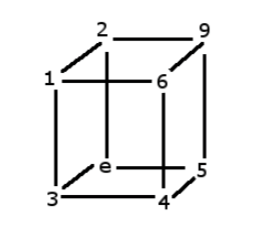
\includegraphics{Figures/hypercube.png}
\decoRule
\caption[hypercube]{3-dimensional hypermatrix(cube).}
\label{fig:hypercube}
\end{figure}

\section{Doubly-Stochastic Matrix}

Doubly Stochastic Matrix is a square matrix of non-negative real numbers, each of whose rows and columns sum to 1. If rows and columns of some matrices sum to n, it can also be considered as doubly stochastic matrix because we can just device all the entries by n, which results to true Doubly Stochastic.\\


Examples:

\[
  \begin{bmatrix}
    0 & 1 & 0 \\
    1 & 0 & 0 \\
    0 & 0 & 1 \\
  \end{bmatrix}
  ,
    \begin{bmatrix}
     1/6 & 5/6 & 0 & 0 \\
     0 & 0 & 1 & 0 \\
     0 & 1/6 & 0 & 5/6 \\
     5/6 & 0 & 0 & 1/6
    \end{bmatrix}
  ,
    \begin{bmatrix}
     \frac{1}{2} & \frac{1}{2} \\
     \frac{1}{2} & \frac{1}{2}
    \end{bmatrix}
\]

\section{Permutation Matrix}

A matrix obtained by permuting the rows of an $n\times n$ identity matrix according to some permutation of the numbers 1 to n. So the number of $n\times n$ permutation matrics is $n!$.\\

The permutation matrics of order 3 are:
\[
  \begin{bmatrix}
    1 & 0 & 0 \\
    0 & 1 & 0 \\
    0 & 0 & 1 \\
  \end{bmatrix}
  ,
    \begin{bmatrix}
     1 & 0 & 0 \\
     0 & 0 & 1 \\
     0 & 1 & 0 \\
    \end{bmatrix}
  ,
    \begin{bmatrix}
     0 & 0 & 1 \\
     1 & 0 & 0 \\
     0 & 1 & 0 \\
    \end{bmatrix}
    ,
    \begin{bmatrix}
     0 & 1 & 0 \\
     1 & 0 & 0 \\
     0 & 0 & 1 \\
    \end{bmatrix}
    ,
    \begin{bmatrix}
     0 & 1 & 0 \\
     0 & 0 & 1 \\
     1 & 0 & 0 \\
    \end{bmatrix}
    ,
    \begin{bmatrix}
     0 & 0 & 1 \\
     0 & 1 & 0 \\
     1 & 0 & 0 \\
    \end{bmatrix}
\]


\section{Polytopes}

In elementary geometry, a polytope is a geometric object with flat sides, and may exist in any general number of dimensions n as an n-dimensional polytope or n-polytope. For example a two-dimensional polygon is a 2-polytope and a three-dimensional polyhedron is a 3-polytope

Mathematically, A polytope $P\subseteq \mathbb{R}^d$ is the convex hull $P=conv(v_1,...,v_k)$ of a finite set of points $v_1,...,v_k \in \mathbb{R}^d$ . Dually any polytope can be written as the bounded intersection of a finite number of affine half-spaces in the form $P = \{ x\mid Ax \leq b \}$

\subsection{Elements of polytope}
A proper face of $F$ of a polytope $P$ is the intersection of $P$ with and affine hyperplane $H$ such that $P$ is completely contained in one of the closed half spaces defined by $H$. The empty set and the polytope P a face of $P$. Any face $F$ is itself  polytope. The dimension of a polytope $P \subseteq \mathbb{R}^d$ is the dimension of the minimum affine space containin it. It is full dimensional if its dimension is d.

0-dimensional faces of $P$ are called $vertices$, 1-dimensional faces are edges. Proper faces of maximal dimensional are called facets. $P$ is the convex hull of its vertices, and the vertices of any face are subset of the vertices of $P$. Thus, a polytope has only a finite number of faces. Let $f_i$ be the number of $i$-dimensional faces of $P,0 \leq i \leq dim P-1$. The $f$-vector of a d-dimensional polytope P is the non-negative integral vector $f(P) = (f_0,...,f_(d-1)$.

The face lattice or combinatorial type $\mathcal{L}(P)$ of a polytope P is the partially ordered set of all faces of P (including the empty face and P itself). This defines Eulerian lattice. Figure shows 2.1 this lattice.


It contains all combinatorial information of the polytope. Two polytopes P,$P'$ are combinatorially isomorphic or have the same combinatorial type if their face lattices are isomorphic as posets.

An r-dimensional simplex (or r-simplex) is the convex hull of r+1 affinely independent points in $\mathbb{R}^d$. A polytope is called simplicial if all facets are simplices. It is simple if the dual is simplicial. Equally, a d-dimensilanl polytope P is simple if each vertex is incident to precisely d edges. The d-dimensional 0/1-cube $C^d$ is the convex hull of all d-dimensinal 0/1-vectors. This is a simple d-polytope with $2^d$ vertices and 2d facets. More generally we denote by a d-cube any d-dimensional polytope that is combinatorially isomorphic to the 0/1-cube (it need not be full dimensional).

\subsection{Properties of Polytope}
Let $P_1 \subset \mathbb{R}^{d_1}$ and $P_2 \subset \mathbb{R}^{d_2}$ be two (geometrically realised) polytopes with vertex sets $V(P_1)=\{ v_1,...,v_k$ and $V(P_2)=\{ w_1,...,w_l \}$. With $0^{(d)}$ we denote he d-dimensional zero vector.

The (geometric) product of $P_1$ and $P_2$ is the polytope

\begin{equation}
P_1 \times P_2 = conv( (v_i,w_i)\in \mathbb{R}^{d_1+d_2}\mid 1\leq i \leq k, i \leq j \leq l)
\label{eqn:Einstein}
\end{equation}

This is the same as the set of all points $(v,w)$ for $v \in P_1$ and $w \in P_2$. The (geometric) join of $P_1$ and $P_2$ is the polytope

\begin{equation}
P_1 \star P_2 := conv(P_1 \times \{ 0^{d_2} \} \times \{ 0 \} \cup \{ 0^{d_1} \} \times P_2 \times \{ 1 \} ) \subseteq \mathbb{R}^{d_1+d_2+1}
\label{eqn:Einstein}
\end{equation}

More generally we say that a polytope P is a product or join of two polytopes $P_1$ and $P_2$, if P is combinatorially isomorphic to the geometric prouct or geometric join of some realisations of the face lattices $P_1$, or $P_2$.

If $F$ is face of a polytope  $P = \{ x \mid Ax \leq b \} \subseteq \mathbb{R}^d$  and $ \langle c,x \rangle \leq d $ a linear funtional defining F, then the $wedge wedge_F(P)$ of P over F is defined to be the polytope.
 
\begin{equation}
wedge_F(P) = \{ (x,x_0) \in \mathbb{R}^{d+1} \mid Ax\leq b, 0\leq x_0 \leq d- \langle c,x \rangle\}
\label{eqn:Einstein}
\end{equation}

Again, we say more generally that P is wedge of a polytope  Q over some face F of Q if P is combinatorially equivalently to $wedge_F(Q)$



%----------------------------------------------------------------------------------------
%	SECTION 2
%----------------------------------------------------------------------------------------

\section{Birkhoff Polytope}

Birkhoff polytope $B_n$ is sometimes considered to be one of the most important polytopes in many sphere. Birkhoff polytope is also called assignment polytope, the polytope of doubly stochastic matrices, or the perfect matching polytope of complete bipartite graph $K_(n,n)$ ,transportation polytope. It surprisingly appears in various branches of mathematics from geometry to enumerative combinatorics to optimisation theory to Statistics.

The Birkhoff polytope $B_n$ is the convex hull of all $(n\times n)$ permutation metrices, i.e.matrices which consists precisely one 1 in every row and column, and zeros at all places. Equivalently, $B_n$ is the set of all non-negative $(n \times n)$-metrices, whose rows and columns all sum to 1, or the perfect matching polytope of the complete bipartite graph $K_(n,n)$. The Birkhoff polytope $B_n$ has dimension $(n-1)^2$ with $n!$ vertices and $n_2$ facets. The Birkhoff-von Neumann Theoram illustrated, $B_n$ can be understood as the intersection of the positive orthant with a family of of hyperplanes.

Birkhoff polytopes are widely studied as a class of polytopes in the area of optimisation, statistics, enumerative combinatorics or representation theory. Despite, Combinatorial and Geometrical structure of Birkhoff polytope and its algorithmic treatment are still open to disover.

A Birkhoff polytope $B_n$ is a polytope defined by the following equations and in-equalities:
\begin{equation}
a_{i,j} \geqslant 0, \sum_{i=1}^{n} a_{i,j} = 1, \sum_{j=1}^{n} a_{i,j}=1 \text{ for all } 1\leqslant i,j\leqslant n.
\label{eqn:Birkhoff_definition}
\end{equation}	

$(a_{i,j}$ can be thought of as  $n\times n$ doubly stochastic matrices. It can be realise that $B_n$ has dimension $(n-1)^2$ as values of $a_{i,j},1\leqslant i,j\leqslant n$ determine the rest. Different way helps to realise that vertices of $P_n$ are permutation matrices.

\section{Properties of $B_n$}
Here I am going to describe some of the properties of Birkhoff polytope.
\subsection{Vetices}
The Birkhoff polytope has $n!$ vertices. This was derived from the Birkhoff-von Neumann theorem.
\subsection{Edges}
The edges of the Birkhoff polytope corresponds to pairs of permutations differing by a cycle:

$(\sigma,\omega)$ such that $\sigma^{-1}\omega$ is a cycle.

This implies that the graph of $B_n$ is a Caley graph of the symmetric group $S_n$. This ialso implies that the graph of $B_3$ is a complete graph $K_6$, and thus $B_3$ is a neighbourly prototype.

\subsection{Facets}
The Birkhoff polytope lies within and $(n^2-2n+1)$-dimensional affine subspace of the $n^2$-dimensional space of all $n\times n$ matrices: this subspace is determined by the linear equality constraints that the sum of each row and each column be one. Within this subspace, it is defined by $n^2$ linear inequalities, one for each coordinate of the matrix, specifying that the coordinate be non-negative. Therefore, it has exactly $n^2$ facets.

\subsection{Symmetries}
The Birkhoff polytop $B_n$ is both vertex-transitive and facet-transitive. This is not regular for $n>2$.

\subsection{Volume}
One of the hardest open problem is to find the volume of a Birkhoff polytopes. Volume calculation was possible for $n\leqslant 10$. It is known to be equal to the volume of polytope associated with standard Young tabuleaux. The following asymptotic formula was founded by Rodney Canifeld and Brenden McKay:

\begin{equation}
vol(B_n)=\exp(-(n-1)^2 \ln n + n^2 - (n-\frac{1}{2} )\ln(2\pi)+\frac{1}{3}+\mathcal{O}(1))
\label{eqn:Birkhoff_volume}
\end{equation}	
% Chapter Template

\chapter{Quadratic Programming} % Main chapter title

\label{ChapterX} % Change X to a consecutive number; for referencing this chapter elsewhere, use \ref{ChapterX}

%----------------------------------------------------------------------------------------
%	SECTION 1
%----------------------------------------------------------------------------------------
An optimisation problem with a quadratic objective function and linear constraints is called a quadratic program. Problem of this type are important in their own right, and they also arise as subproblems in methods for general constrained optimisations. 

\section{Definition of QP}

The general quadratic program(QP) can be stated as

\begin{equation}
\begin{aligned}
& \underset{x}{\text{min}}
& & q(x)= \frac{1}{2}x^{T}Gx+x^{T}c \\
& \text{subject to} & &  a_{i}^{T}x = b_i & i\in \mathbb{E} \\
& & &  a_i^{T}x \geqslant b_{i} & i\in \mathbb{I}
\end{aligned}
\label{eqn:quadratic_programming}
\end{equation}
where $G$ is a symmetric $n\times n$ matrix, $E$ and $I$ are finite sets of indices, and $c$,$x$, and $a_i, i\in E \cup I$, are vectors in $\mathbb{R}^n$. Quadratic programs can always be solved (or shown to be infeasible) in a finite amount of computation, but the effort required to find a solution depends strongly on the characteristics of the objective function and the number of inequality constraints. If the Hessian matrix $G$ is positive semidefinite, we say that \ref{eqn:quadratic_programming} is a convex QP, and in this case the problem is often similar in difficulty to a linear program. (Strictly convex QPs are those in which G is positive definite.) Nonconvex QPs, in which G is an indefinite matrix, can be more challenging because they can have several stationary points and local minima.

In this chapter we will try to show different kinds of quadratic programs but we will mainly focus on convex quadratic program and different algorithms of convex quadratic programs.

\section{Classification of QP's}

Some classification of quadratic program's:
\begin{itemize}
	\item Unconstrianed QP
	\item Box constrained QP
	\item Equality constrained QP
	\item Inequality constrained QP.
\end{itemize}

\section*{Important Definitions}
\subsection*{Logarithmic barrier}
Consider inequalities $Ax \leqslant b$ with $A$ of size $m\times n$ and with rows $a_i^T$. Define
\begin{equation*}
P=\lbrace x \mid Ax \leqslant b \rbrace \text{ and } P^0=\lbrace x \mid Ax < b \rbrace
\end{equation*}
logarithmic barrier for the inequalities $Ax\leqslant b$:
\begin{equation*}
\begin{aligned}
	\phi(x) = - \sum_{i=1}^{m}\log(b_i - a_i^Tx) & & \text{with domain } P^0
\end{aligned}	
\end{equation*}
\begin{figure}[h]
\centering
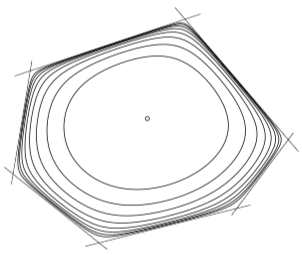
\includegraphics[scale=0.5]{Figures/logarithmic_barrier.png}
\decoRule
\caption[hypercube]{Logarithmic barrier function.}
\label{fig:logarithmic_barrier}
\end{figure}


\subsection*{Gradient}
Gradient $\nabla \phi(x)$ is the n-vector with $\nabla \phi(x)_i = \frac{\delta \phi (x)}{\delta x_i}$
\begin{equation*}
	\begin{aligned}
		\nabla \phi(x) = \sum_{k=1}^{m} \frac{1}{b_k-a_k^Tx}a_k = A^Td_x 
	\end{aligned}
\end{equation*}
$d_x$ denotes the positive $m-$vector
\begin{equation*}
	\begin{aligned}
		d_x = \left( \frac{1}{b_1-a_1^Tx},..., \frac{1}{b_m-a_m^Tx} \right)
	\end{aligned}
\end{equation*}


\subsection*{KKT System}
KKT System is

\subsection*{Hessian Matrix}
Hessian Matrix Gradient $\nabla^2 \phi(x)$ is the $n\times n$-matrix with $\nabla \phi (x)_{ij} = \frac{\delta^2 \phi (x)}{\delta x_i \delta x_j}$

\begin{equation*}
	\begin{aligned}
		\nabla^2 \phi(x) = \sum_{k=1}^{m} \frac{1}{(b_k-a_k^Tx)^2} a_k a_k^T = A^T diag(d_x)^2 A 
	\end{aligned}
\end{equation*}

\subsection*{Central Path}
Consider the linear programming problem in standard form:
\begin{equation*}
\begin{aligned}
\text{min } c^Tx, & & \text{subject to} Ax=b, \geqslant 0	
\end{aligned}
\end{equation*}
where $c$ and $x$ are vectors in $\mathbb{R}^n$, b is a vector in $\mathbb{R}^m$, and $A$ is an $m\times n$ matrix with full row rank. The dual problem of the above problem is
\begin{equation*}
\begin{aligned}
	\text{max } b^T\lambda, & & \text{subject to} A^T\lambda + s = c, x\geqslant 0
\end{aligned}
\end{equation*}
where $\lambda$ is a vector in $\mathbb{R}^m$ and s is a vector in $\mathbb{R}^n$
The primal-dual feasible set $\mathcal{F}$ and strictly feasible set $\mathcal{F}^0$ are defined as
\begin{equation*}
	\begin{aligned}
		\mathcal{F} &= \lbrace (x,\lambda,s) \mid Ax=b, A^T\lambda +s = c, (x,s) \geqslant0 \rbrace\\
		\mathcal{F}^0 &= \lbrace (x,\lambda,s) \mid Ax=b, A^T\lambda +s = c, (x,s) > 0 \rbrace
	\end{aligned}
\end{equation*}
The central path $C$ is an arc of strictly feasible points. It is parameterized by a scalar $\eta > 0$, and each point $(x_\tau ,\lambda_\tau, s_\tau)\in \mathcal{C}$ satisfies the following equations:
\begin{equation*}
	\begin{aligned}
		A^T\lambda+s &= c,\\
		Ax &= b,
		x_i,s_i &= \tau & & i = 1,2,...n.\\ 
		(x,s ) & > 0.
	\end{aligned}
\end{equation*}
So the central path is defined as:
\begin{equation*}
\begin{aligned}
	\mathcal{C} = \lbrace (x_\tau,\lambda_\tau, s_\tau)\mid \tau>0\rbrace
\end{aligned}
\end{equation*}
Another way of defining $\mathcal{C}$ is:
\begin{equation*}
\begin{aligned}
F(x_\tau,\lambda_\tau, s_\tau)=
	\begin{bmatrix}
		0\\
		0\\
		\tau e
	\end{bmatrix},
	(x_\tau,s_\tau) > 0
\end{aligned}
\end{equation*}

the conditions approximate more and more colsely as $\tau$ goes to zero. If $\mathcal{C}$ converges to anything as $\tau \downarrow 0$, it must converge to a primal-dual solution of the linear program.


\subsection*{Active set}
The Active set $\mathbb{A}(x)$ at any feasible $x$ consists of the equality constraint indices from $\varepsilon$ together with the indices of the inequality constraints $i$ for which $c_i(x)=0$; that is,
\begin{equation*}
	\begin{aligned}
		\mathbb{A}(x)=\varepsilon \cup {i\in \mathbb{I}\mid c_i(x)=0}
	\end{aligned}
\end{equation*}
At a feasible point x, the inequality constraint $i\in \mathbb{I}$ is said to be active if $c_i(x)=0$ and inactive if the strict inequality $c_i(x)>0$ is satisfied.

\section{Equality-Constrained Quadratic Programs}

We start this section with of algorithms for quadratic programming by considering the case of equality constrained

\subsection*{Properties of Equality-constrained QPs}
To make it simple, we write the equality constraint in a form of matrix and define it as follows:

\begin{equation}
\begin{aligned}
& \underset{x}{\text{min}}
& & q(x)= \frac{1}{2}x^{T}Gx+x^{T}c \\
& \text{subject to} & &  Ax=b
\end{aligned}
\label{eqn:equality_constrained_QP}
\end{equation}

where $A$ is the $m\times n$ Jacobian of constraints (with $m\leqslant n$) whose rows are $a_i^T,i \in \mathbb{E}$ and $b$ is the vecotor in $\mathbb{R}^n$ whose componants are $b_i, i \in \mathbb{E}$. Currently, we consider that $A$ has a full row rank (rank m) so that the constraints are consistent.

The first-order necessary conditions for $x^*$ to be a solution of \ref{eqn:equality_constrained_QP} state that there is a vector $\lambda^*$ such that the following system of equations is satisfied:

\begin{equation}
\begin{bmatrix}
  	G & -A^T \\
    A & 0
  \end{bmatrix}
  \begin{bmatrix}
  	x^* \\
    \lambda{*}
  \end{bmatrix}
  =
  \begin{bmatrix}
  	-c \\
    b
  \end{bmatrix}	
  \label{eqn:Properties_of_EC_QP}
\end{equation}

These conditions are a consequence of the general result for first-order optimality conditions.  $\lambda^*$ is called the vector of Lagrange multipliers. In \ref{eqn:Properties_of_EC_QP} we can write $x^*$ as $x^* = x+p$ which makes it useful for computation, where x is some estimate of the solution and p is the desired step. By introducing this and rearranging the equations, we obtain

\begin{equation}
\begin{bmatrix}
  	G & A^T \\
    A & 0
  \end{bmatrix}
  \begin{bmatrix}
  	-p \\
    \lambda{*}
  \end{bmatrix}
  =
  \begin{bmatrix}
  	g \\
    h
  \end{bmatrix}	
  \label{eqn:Properties_of_EC_QP_2}
\end{equation}
where
\begin{equation}
\begin{aligned}
h= Ax-b, & g = c+Gx, & p = x^* - x.
\end{aligned}
\label{eqn:Properties_of_EC_QP_3}	
\end{equation}

The matrix \ref{eqn:Properties_of_EC_QP_2} is called the Karush-Kuhn-Tucker (KKT) matrix, and the following result gives conditions under which it is nonsingular. We will use $Z$ to denote the $n \times (n-m)$ matrix whose columns are basis for the null space of $A$. That is, $z$ has full  rank and satisfies $AZ=0$.

\begin{mybox}{Lemma}
\begin{lemma}
\textit{Let $A$ have full row rank, and assume that the reduce Hessian matrix $Z^TGZ$ is positive definite. Then the KKT matrix}

\begin{equation}
	\begin{bmatrix}
  		G & A^T \\
    	A & 0
    \end{bmatrix}
\label{eqn:Properties_of_EC_QP_4}	
\end{equation}
\textit{is nonsingular, and hence there is a unique vector pair $(x^*, \lambda^*)$ satisfying \ref{eqn:Properties_of_EC_QP}}.	
\label{lemma:KKT_nonsingularuty}
\end{lemma}
\end{mybox}

So, when the conditions of the \ref{lemma:KKT_nonsingularuty} is satisfied, there is a unique vector pair $(x^*, \lambda^*)$ that satiesfies the first-order necessary condition for \ref{eqn:equality_constrained_QP}. In fact, the second order sufficient conditions are also satisfied at $(x^*, \lambda^*)$, so $x^*$ is a strict local minimizer of \ref{eqn:equality_constrained_QP}. In fact we can use a direct argument to show that $x^*$ is a global solution of \ref{eqn:equality_constrained_QP}.

\begin{mybox}{Theorem}
\begin{theorem}
	Let A have full row rank and assume that the reduced-Hessian matrix $Z^TGZ$ is positive definite. Then the vector $x^*$ satisfying \ref{eqn:Properties_of_EC_QP} is the unique global solution of \ref{eqn:equality_constrained_QP}.
\end{theorem}
\end{mybox}
\begin{proof}
	Let x be any other feasible point (satisfying $Ax=b$), and as before, let $p$ denote the difference $x^*-x$. Since $Ax^*=Ax=b$, we have that $Ap=0$. By substituting into the objective function \ref{eqn:equality_constrained_QP}, we get
	\begin{equation}
	\begin{aligned}
		q(x) & = \frac{1}{2}(x^*-p)^TG(x^*-p)+C^T(x^*-p)\\
		& = \frac{1}{2}p^TGp-p^TGx^*-C^Tp+q(x^*)
	\end{aligned}
	\label{eqn:Properties_of_EC_QP_5}
	\end{equation}
	From \ref{eqn:Properties_of_EC_QP} we have that $Gx^*=-c+A^T\lambda^*$, so from $Ap = 0$ we have that
	\begin{equation}
	\begin{aligned}
		p^TGx^* &= p^T(-c)+A^T\lambda^* = -p^Tc.
	\end{aligned}
	\label{eqn:Properties_of_EC_QP_6}
	\end{equation}
	By substituting this relation into \ref{eqn:Properties_of_EC_QP_5}, we obtain
	\begin{equation}
	\begin{aligned}
		q(x)= \frac{1}{2} p^TGp + q(x^*).
	\end{aligned}
	\label{eqn:Properties_of_EC_QP_7}
	\end{equation}
	Since $p$ lies in the null space of $A$, we can write $p=Zu$ for some vector $u\in \mathbb{R}^{n-m}$, so that
	\begin{equation}
	\begin{aligned}
		q(x)= \frac{1}{2} u^TZ^TGZu + q(x^*).
	\end{aligned}
	\label{eqn:Properties_of_EC_QP_8}
	\end{equation}
	By positive definiteness of $Z^TGZ$, we conclude that $q(x)>q(x^*)$ except when $u=0$, that is, when $x=x*$. Therefore, $x^*$ is the unique global solution of \ref{eqn:equality_constrained_QP}
\end{proof}

When the reduced Hessian matrix $Z^TGZ$ is positive semidefinite with zero eigenvalues, the vector $x^*$ satisfying \ref{eqn:Properties_of_EC_QP_2} is a local minimizer but not a strict local minimizer. If the reduced Hessian has negative eigenvalues, then $x^*$ is only a stationary point, not a local minimizer.

\section{Direct Solution of the KKT System}

In this section we discuss the efficient methods of solving KKT system. The KKT system is always indefinite if $m\geqslant1$. We can apply direct techniques to solve indefinite KKT system.

\subsection*{Factoring the Full Scale System}
One option for solving KKT system is to perform triangular factorization on the full KKT matrix and then perform backward and forward substitution with the triangular factors. It is not possible to apply Cholesky factorization as it is indefinite.Another option can be Gaussian Elimination to obtain the $L$ and $U$ factors, but this method does not consider the symmetry.

So, the most effective strategy is to use symmetric indefinite factorization which has the form of:

\begin{equation}
	\begin{aligned}
		P^TKP = LDL^T
	\end{aligned}
	\label{eqn:SIF_1}
\end{equation}
where $P$ is an appropriately chosen permutation matrix. $L$ is lower triangular with $diag(L) = I$ and $D$ is block diagonal.
Based on \ref{eqn:SIF_1}, the KKT system \ref{eqn:Properties_of_EC_QP_2} is solved as follows:
\begin{equation}
	\begin{aligned}
		solve & & Ly = P^T
		\begin{bmatrix}
  		g \\
    	h
    \end{bmatrix}\\
    solve & & D\hat{y} = y\\
    solve & & L^T\bar{y} = \hat{y}\\
    set & & \begin{bmatrix}
  		-p \\
    	\lambda^*
    \end{bmatrix} = P\bar{y}
	\end{aligned}
	\label{eqn:SIF_2}
\end{equation}

This approach of factoring  the full $(n+m)\times (n+m)$ KKt matrix is quite effective  on many problems. It can be expensive when the permutation matrix $P$ are not able to maintain sparsity in the $L$ factor.
\subsection*{Range-space approach}
The range-space approach is useful when $G\in \mathbb{R}^{n\times n}$ is symmetric positive definite. We can multiply the first part of the equation \ref{eqn:Properties_of_EC_QP_2}  by $AG^-1$ and then subtract the second part to obtain a linear system in the vector $\lambda^*$ alone:

\begin{equation}
	\begin{aligned}
		(AG^{-1}A^T\lambda^*) = (AG^{-1}g-h)
	\end{aligned}
	\label{eqn:Range_space_1}
\end{equation}

We solve this symmetric semidifinite system for $\lambda^*$ and then recover $p$ from the first equation in \ref{eqn:Properties_of_EC_QP_2} by solving
\begin{equation}
	\begin{aligned}
		Gp = A^T\lambda^*-g
	\end{aligned}
	\label{eqn:Range_space_2}
\end{equation}

This approach requires us to perform operation with $G^{-1}$, as well as to compute the factorization of the $m\times n$ matrix $AG^{-1}A^T$. That is why it is useful when:
\begin{itemize}
	\item G is well conditioned and easily invertible (e.g., G is diagonal or block-diagonal),
	\item $B^{-1}$ is known explicitely (e.g., by means of a quasi-Newton updating formula),
	\item the number $m$ of equality constraints is small.
\end{itemize}

\subsection*{Null-space approach}
The null-space approach does not require regularity of $G$ and thus has a wider range of applicability than the range-space approach.

We assume that $A\in \mathbb{R}^{m\times n}$ has full row rank m and that $Z^TGZ$ is positive definite, where $Z\in \mathbb{R}^{n\times (n-m)}$ is the matrix whose columns span Ker $A$ which can be computed by QR factorization.

We partition the vector $x^*$ according to
\begin{equation}
	\begin{aligned}
		x^* = Yw_y + Zw_z
	\end{aligned}
	\label{eqn:Null_space_1}
\end{equation}
where $Y\in \mathbf{R}^{n\times m}$ is such that $[Y\quad Z]\in \mathbb{R}^{n\times n}$ is nonsingular and $w_y \in \mathbb{R}^m,w_Z \in \mathbb{R}^{n-m}$.

Substituting \ref{eqn:Null_space_1} into the \ref{eqn:Properties_of_EC_QP_2}, we get
\begin{equation}
	\begin{aligned}
		Ax^* = AYw_Y + AZw_Z = c\\
		AZ=0
	\end{aligned}
	\label{eqn:Null_space_2}
\end{equation}
i.e., $Yw_Y$ is a particular solution of $Ax=c$.

Since $A\in \mathbb{R}^{m\times n}$ has rank $m$ and $[Y \quad Z]\in \mathbb{R}^{n\times n}$ is nonsingular, the product matrix $[Y \quad Z] = [AY \quad 0]\in \mathbb{R}^{m\times m}$ is non singular. Hence, $w_Y$ is well determined by \ref{eqn:Null_space_2}.

On the otherhand, substituting \ref{eqn:Null_space_1} into the first equation of \ref{eqn:Properties_of_EC_QP_2}, we get
\begin{equation}
	\begin{aligned}
		GYw_Y + GZw_Z + A^T\lambda^* = b.
	\end{aligned}
	\label{eqn:Null_space_3}
\end{equation}
Multiplying by $Z^T$ and observing $Z^{T}A^{T}=(AZ)^T=0$ yields
\begin{equation}
	\begin{aligned}
		Z^TGZw_Z = Z^Tb - Z^TGY w_Y.
	\end{aligned}
	\label{eqn:Null_space_4}
\end{equation}

The reduced KKT system \ref{eqn:Null_space_4} can be solved by a Cholesky factorization of the reduced Hessian $Z^TBZ\in \mathbb{R}^{(n-m)\times(n-m)}$. Once $w_Y$ and $w_Z$ have been computed as the solution of \ref{eqn:Null_space_3} and \ref{eqn:Null_space_3}, $x^*$ is obtained according to \ref{eqn:Null_space_1}.

Finally, the Lagrange multiplier turns out to be the solution of the linear system arising from multiplication of the equation \ref{eqn:Null_space_1} by $Y^T$:
\begin{equation}
	\begin{aligned}
		(AY)^T\lambda^* = Y^Tb - Y^TGx^*
	\end{aligned}
\end{equation} 


\section{Iterative solution of the KKT system}
Direct solution of the KKT system can be sometimes expensive, the possible alternative is iterative method to solve KKT system. one of the famous iterative method is Conjugate Gradient method. Although it is not recommended for solving the full system using the CG mathod because it can be unstable on systems that are not positive definite. An iterative solver can be applied either to the entire KKT system or, as in the null-space and range-space approach, use the special structure of the KKT matrix.

\section{Inequality-Constrained Problems}
Inequality-constrained quadratic programs are QPs which consists of inequality constraints and may or may not consist equality constraints. Several classes of algorithms for solving convex quadratic programs containing inequality and equality constraints are available. Active-set method and Interior-point are most famous for their accuracy and capability to solve large problems.

\subsection{Properties of Inequality-constrained problems}
\subsubsection*{Optimality condition for inequality-constrained problems}
Lagrangian for the problem \ref{eqn:quadratic_programming} is:
\begin{equation}
	\begin{aligned}
		\mathcal{L}(x,\lambda ) = \frac{1}{2}x^TGx + x^Tc-\sum_{i\in \mathcal{I}\cup \varepsilon} \lambda_i(a_i^Tx-b_i)
	\end{aligned}
	\label{eqn:Lagrangian_for_QP_1}
\end{equation}

The active set $\mathcal{A}(x^*)$ consists of indices of the constraints for which equality holds at $x^*$:
\begin{equation}
	\begin{aligned}
		\mathcal{A}(x^*) = \lbrace i\in \varepsilon \cup \mathcal{I}\mid a_i^Tx^* = b_i \rbrace
	\end{aligned}
\end{equation}

According to the KKT condition for this problem, it is found that any solution $x^*$ for some Lagrange multipliers $\lambda_i^*, i\in \mathcal{A}(x^*)$ of \ref{eqn:quadratic_programming} satisfies the following conditions:
\begin{equation}
	\begin{aligned}
		Gx^*+c-\sum_{i\in \mathcal{A}(x^*)} \lambda_i^*a_i &= 0\\
		a_i^Tx^* &= b_i & & \text{for all }i\in \mathcal{A}(x^*),\\
		a_i^Tx^* &\geqslant b_i & & \text{for all }i\in \mathcal{I} \slash \mathcal{A}(x^*),\\
		\lambda_i^* &\geqslant 0 , & & \text{for all }i\in \mathcal{I} \cap \mathcal{A}(x^*),\\
	\end{aligned}
	\label{eqn:KKT_condition_for_convex_QP}
\end{equation}

Incase of convex QP, that is when $G$ is positive semidefinite, \ref{eqn:KKT_condition_for_convex_QP} are sufficient for $x^*$ to be a global solution.

\begin{mybox}{Theorem}
\begin{theorem}
	If $x^*$ satisfies the conditions \ref{eqn:KKT_condition_for_convex_QP} for some $\lambda_i^*,i \in \mathcal{A}(x^*)$, and $G$ is positive semidefinite, then $x^*$ is a global solution of \ref{eqn:quadratic_programming}.
\end{theorem}
\end{mybox}

\subsubsection*{Degeneracy}
Degeneracy initiates difficulties for some optimisation algorithm. It appears in the following situation:
\begin{itemize}
	\item the active constraint gradients $a_i,i\in \mathcal{A}(x^*)$, are linearly dependent at the solution $x^*$, and/or
	\item there is some index $i\in \mathcal{A}(x^*)$ such that all Lagrange multipliers satifying KKT conditions have $\lambda_i^* = 0$
	
	\begin{figure}[h]
		\centering
			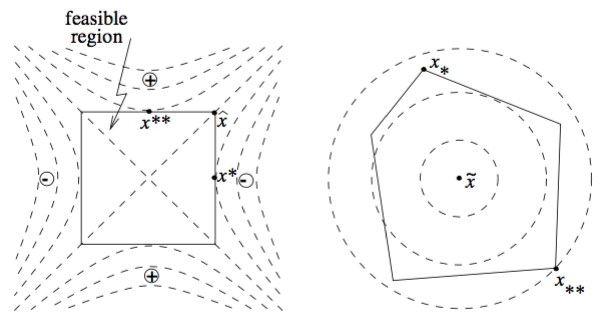
\includegraphics[scale=0.5]{Figures/Degeneracy_2.png}
			\decoRule
			\caption[hypercube]{Nonconvex quadratic programs.}
		\label{fig:Degeneracy_1}
	\end{figure}
	\begin{figure}[h]
		\centering
			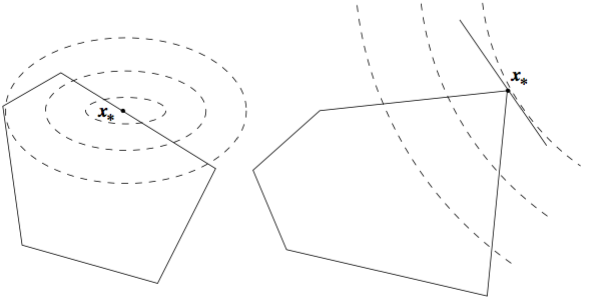
\includegraphics[scale=0.5]{Figures/Degeneracy_1.png}
			\decoRule
			\caption[hypercube]{Degenerate solutions of quadratic programs.}
		\label{fig:Degeneracy_2}
	\end{figure}
\end{itemize}
In the figure \ref{fig:Degeneracy_2} two instances are visualized. There is only a single active constraint at the solution $x^*$ in the left picture, that is lso an unconstrained minimizer of the objective function. According to KKT condition, $Gx^*+c=0$, such that the lone Lagrange multiplier should be zero.  3 constraints are active at the solution $x^*$ in the right-side image. As each of the three constraint gradients is a a vector in $\mathbb{R}^2$, they should be linearly independent.

Specifically for two reason Degeneracy can cause problems for optimization algorithms,
\begin{itemize}
	\item First linear dependence of the active constraint gradients can cause numerical difficulties as several matrices which required to factor become rank deficient.
	\item Second when the problem contains weakly active constraints, it is difficult for the algorithm to determine whether these constraints are active at the solution.
\end{itemize} 





\section{Active-set Methods for Convex QPs}
Active-set methods are important method for solving convex quadratic programs which consists equality and inequality constraints. Active set method starts by finding a feasible point during initial phase and then search for a solution along the edges and faces of the feasible set by solving a sequence of equality-constrained QPs.

If it was possible to know the contents of the active set earlier, it would be straight forward to get the solution by solving an equality-constrained QP of the form:
\begin{equation*}
	\begin{aligned}
		& \underset{x}{\text{min}} & & q(x)= \frac{1}{2}x^{T}Gx+x^{T}c \\
& \text{subject to} & &  a_{i}^{T}x = b_i & \forall i\in \mathcal{A}(x^*)
	\end{aligned}
\end{equation*}
But usually it is not possible to know $\mathcal{A}(x^*)$ and termination of this set is a major challnage for algorithms.

Primal active-set method follows step from one iteration to another by solving a quadratic subproblem in which some of the equality constraints and all the inequality constraints are imposed as equalities which is referred to as the working set. Working set at $k$th iterate $x_k$ is denoted by $\mathcal{W}_k$

Consider an iterate $x_k$ and the working set $\mathcal{W}_k$, it is necessary to check if $x_k$ minimizes the quadratic $q$ in the subspace defined by working set. Otherwise step p is computed by solving an equality-constrained subproblem in which the constraints corresponding to the working set $\mathcal{W}_k$ are regarded as equalities and all other constraints are temporarily disregarded. We define this subproblem in terms of the step p:
\begin{equation*}
	\begin{aligned}
		p = x - x_k, & & g_k = Gx_k + c.
	\end{aligned}
\end{equation*}

By substituting $x$ with $(x_k+p)$ into \ref{eqn:quadratic_programming},
\begin{equation*}
	\begin{aligned}
		q(x) = q(x_k+p)= \frac{1}{2}p^TGp+g_k^Tp+\rho_k
	\end{aligned}
\end{equation*}
$\rho_k$ is independent of p. So without considering $\rho_k$, we can write the QP subproblem to be solved at $k$th iteration as:

\begin{equation}
	\begin{aligned}
		& \underset{x}{\text{min}} & & \frac{1}{2}p^{T}Gp+g_{k}^{T}p \\
& \text{subject to} & &  a_{i}^{T}p = 0 & \forall i\in \mathcal{W}_k
	\end{aligned}
	\label{eqn:Active_set_1}
\end{equation}

Solution of this subproblem is denoted by $p_k$. Consider optimal $p_k$ is nonzero for the moment. We need to calculate displacement along this direction. If $x_k+p_k$ is feasible with respect to all the constraints, then we can set:
\begin{equation*}
\begin{aligned}
	x_{k+1} = x_k + p_k
\end{aligned}
\end{equation*} 
Otherwise, we set:
\begin{equation}
	\begin{aligned}
		x_{k+1} = x_k + \alpha_{k}p_{k}
	\end{aligned}
	\label{eqn:Active_set_2}
\end{equation}
Where $\alpha_k$ is the step length and is chosen possible largest value in the range $[0,1]$ for which all constraints are satisfied.

\subsection*{Selecting $\alpha_k$}
If $a_{i}^{T}p_{k} \geqslant 0$ for some $i\notin \mathcal{W}_k$, then for all $\alpha_k \geqslant 0$ we have $a_{i}^T(x_k+\alpha_kp_k)\geqslant a_{i}^Tx_k \geqslant b_i$. So, constraint $i$ will be satisfied for all nonnegative choices of the step-length parameter. Whenever $a_i^Tp_k < 0$ for some $i\notin \mathcal{W}_k$, we have  $a_{i}^T(x_k+\alpha_kp_k) \geqslant b_i$ only if
\begin{equation*}
	\begin{aligned}
		\alpha_k \leqslant \frac{b_i-a_i^Tx_k}{a_i^Tp_k}
	\end{aligned}
\end{equation*}
So, to maximize the decrement of q, $\alpha_k$ should be as large as possible in $[0,1]$ subject to retaining feasibility, so we get the following equation:

\begin{equation}
	\begin{aligned}
		\alpha_k = {\text{min}} \left( 1, \underset{i\notin \mathcal{W}_k,a_i^Tp_k<0 }{\text{min}} \frac{b_i-a_i^Tx_k}{a_i^Tp_k} \right) 
	\end{aligned}
	\label{eqn:Active_set_3}
\end{equation}

The constraints $i$ for which the minimum is achieved called blocking constraints. 

If $\alpha_k = 1$ and no new constraints are active at $ x_k+\alpha_kp_k $, then there is no blocking constraints on this iteration. 

If $\alpha_k < 1$, step along $p_k$ was blocked by some constraints not in $\mathcal{W}_k$, $\mathcal{W}_{k+1}$ is built by adding one of the blocking constraints to $\mathcal{W}_k$

This method is repeated untill a point $\hat{x}$ has been achieved that minimizes the quadratic objective function over its current working set $\hat{\mathcal{W}}$. Identifying this point is not hard because the subproblem as solution $p=0$. Since $p=0$ satisfies the optimality condition \ref{eqn:Properties_of_EC_QP_2} for \ref{eqn:Active_set_1}, it is found that:

\begin{equation}
	\begin{aligned}
		\underset{i\in \hat{\mathcal{W}}}{\sum}a_i\hat{\lambda}_i = g = G\hat{x}+c
	\end{aligned}
	\label{eqn:Active_set_4}
\end{equation}

for some Lagrange multipliers $\hat{\lambda}_i,i \in \hat{\mathcal{W}}$.  It follows that $x^*$ and $\lambda^*$ satisfy the first KKT condition, if the multipliers are defined corresponding to the inequality constraints that are not in the working set to be zero. As there are some control imposed on the step length, $x^*$ is also feasible with respect to all the constraints, so the second and third KKT conditions are satisfied at this point.\\

Considering the signs of the multipliers corresponding to the inequality constraints in the working set, that is, the indices $i\in \hat{\mathcal{W}} \cap \mathcal{I}$. The fourth KKT condition is also satisfied if these multipliers are all nonnegative. So it can be concluded that, $\hat{x}$ is a KKT point for the original problem \ref{eqn:quadratic_programming}. In fact, since G is positive semidefinite, we have from Theorem *** that $\hat{x}$ is a global solution of \ref{eqn:quadratic_programming}.

If on the other hand, if there exists some $j \in \hat{\mathcal{W}}\cap \mathcal{I}$, such that
\begin{equation*}
	\begin{aligned}
		\lambda^* < 0
	\end{aligned}
\end{equation*}

That constraints has to be removed from the active set and solve new subproblem. This will decreases the objective function. The following theorem states that this strategy produces a direction $p$ at the next iteration  that is feasible with respect to the removed constraint.
\begin{mybox}{Theorem}
\begin{theorem}
	Suppose that the point $\hat{x}$ satisfies first-order conditions for the equality-constrained subproblem with working set $\hat{W}$; that is, equation \ref{eqn:Active_set_3} is satisfied along with $a_i^T\hat{x}=b_i$ for all $i\in \hat{W}$ . Suppose, too, that the constraint gradients $a_i,i\in \hat{W}$, are linearly independent and that there is an index $j\in \hat{W}$ such that $\hat{lambda}_j<0$. 
	
	Let $p$ be the solution obtained by dropping the constraint $j$ and solving the following subproblem:
	\begin{equation}
	\begin{aligned}
		& \underset{p}{\text{min}} & & \frac{1}{2}p^{T}Gp+(G\hat{x}+c)^{T}p, \\
& \text{subject to} & &  a_{i}^{T}p = 0 & \forall i\in \hat{\mathcal{W}} \text{ with } i\neq j
	\end{aligned}
	\label{eqn:Active_set_5}
\end{equation}
Then $p$ is a feasible direction for constraint $j$,that is, $a_j^Tp \geqslant 0$. Moreover,if $p$ satisfies second- order sufficient conditions for above equation, then we have that $a_j^T > 0$, and that $p$ is a descent direction for $q(.)$.
\end{theorem}
\end{mybox}
Whenever $p_k$ obtained from \ref{eqn:Active_set_1} is nonzero and satisfies second-order sufficient optimality conditions for the current working set, it is a direction of strict descent for $q(.)$


\begin{mybox}{Theorem}
\begin{theorem}
	Suppose that the solution $p_k$ of \ref{eqn:Active_set_1} is nonzero and satisfies the second order sufficient conditions for optimality for that problem. Then the function $q(.)$ is strictly decreasing along the direction $p_k$ .
\end{theorem}
\end{mybox}

So it can be concluded that, When G is positive definite-the second order sufficient conditions are satisfied for all feasible subproblems of the form \ref{eqn:Active_set_1}. Hence, it follows from the result that a strict decrease in $q(.)$ can be obtained whenever $p_k \neq 0$.

\subsection*{Specification of the Active-set method for convex QP}
The whole Active-set algorithm can be specified as following:
\begin{algorithm}[h]
  \caption{Active-set method for convex QP}\label{euclid}
  \begin{algorithmic}[1]
    \Procedure{ActiveSet}{}
      \State Compute a feasible starting point $x_0$;
      \State Set $\mathcal{W}_0$ to be a subset of the active constraints at $x_0$;
      \For{\texttt{$k=0,1,2,...$}}
        \State Solve \ref{eqn:Active_set_1} to find $p_k$;
        \If{$p_k==0$}
          \State Compute Lagrange multipliers $\hat{\lambda}$ that satisfy \ref{eqn:Active_set_1} with $\hat{\mathcal{W}}==\mathcal{W}_k$
          \If{$\hat{\lambda} \geqslant 0$} for all $i \in \mathcal{W}\cap \mathcal{I}$
          	\State Stop with solution $x^* = x_k$
          \Else
          	\State $j \gets argmin_{j\in \mathcal{W}_k \cap \mathcal{I}}$ $\hat{\lambda}_j$
          	\State $x_{k+1} \gets x_k$
          	\State $\mathcal{W}_{k+1} \gets \mathcal{W}_k\backslash \lbrace{j \rbrace}$
          \EndIf 
        \Else
          \State $\alpha_k$ from \ref{eqn:Active_set_3}
          \State $x_{k+1} \gets x_k + \alpha_kp_k$
          \If{there are blocking constraints}
          	\State obtain $\mathcal{W}_{k+1}$ by adding one of the blocking constraints to $\mathcal{W}_k$
          \Else
          	\State $\mathcal{W}_{k+1} \gets \mathcal{W}_k$  
          \EndIf
        \EndIf
      \EndFor
    \EndProcedure
  \end{algorithmic}
\end{algorithm}

To implement active-set method efficiently an important key is reuse of nformation from solving the equality-constrained subproblem at the next iteration. The only difference between two consecutive subproblems is that the working set grows or shrinks by a single component. Efficient codes perform updates of the matrix factorizations obtained at the previous iteration, rather than calculating them from scratch each time.



\section{Interior-Point Method}
Interior-point methods follow iterative approach which is a good candidate as alternative of active-set method. This method is also know as trajectory-following, path-following method. 
Here only convex quadratic programming problem with inequality constraints will be focused. It is easier to the problem as follows:

\begin{equation}
\begin{aligned}
& \underset{x}{\text{min}}
& & q(x)= \frac{1}{2}x^{T}Gx+x^{T}c \\
& \text{subject to} & &  Ax \geqslant b
\end{aligned}
\label{eqn:Path_following_1}
\end{equation}

where $G\in \mathbb{R}^{n\times n}$ is symmetric, positive semidefinite, $A\in \mathbb{R}^{m\times n}$.
\begin{equation*}
	\begin{aligned}
		A = [a_i]_{i\in \mathcal{I}} & & b = [b_i]_{i\in \mathcal{I}}, & & \mathcal{I}=\lbrace 1,2,3...,m \rbrace 
	\end{aligned}
\end{equation*}

KKT conditions for this notation can be written as follows:
\begin{equation}
	\begin{aligned}
		Gx- A^T\lambda + c &= 0,\\
		Ax - b  &\geqslant 0, \\
		(Ax-b)_i\lambda_i &= 0, & & i = 1,2,...,m\\
		\lambda &\geqslant 0.
	\end{aligned}
	\label{eqn:Path_following_2}
\end{equation}
By introducing the slack vector $y \geqslant 0$, conditions can be rewritten as:
\begin{equation}
	\begin{aligned}
		Gx- A^T\lambda + c &= 0,\\
		Ax - y - b  &= 0, \\
		y_i\lambda_i &= 0, & & i=1,2,...,m\\
		(y,\lambda) \geqslant 0,
	\end{aligned}
	\label{eqn:Path_following_3}
\end{equation}

As $G$ is positive semidefinite, above KKT conditions are necessary and sufficient to solve convex quadratic program.

Let, current iterate $(x,y,z)$ that satisfies $(y,\lambda)>0$, a complementary measure $\mu$ can be defined as:
\begin{equation}
	\begin{aligned}
		\mu = \frac{y^T\lambda}{m}
	\end{aligned}
	\label{eqn:Path_following_4}
\end{equation}
Derived path-following for the KKT conditions by considering the above KKT conditions:

\begin{equation}
\begin{aligned}
F(x,y,\lambda:\sigma,\mu) = 
\begin{bmatrix}
  	Gx-A^T\lambda+c\\
    Ax-y-b\\
    \mathcal{Y} \Lambda e - \sigma \mu e
  \end{bmatrix}
  =0
\end{aligned}
\label{eqn:Path_following_5}
\end{equation}

Where
\begin{equation*}
	\begin{aligned}
		\mathcal{Y} = diag(y_1,y_2,...,y_m), & & \Lambda = diag(\lambda_1 , \lambda_2,...,\lambda_1), & & e = (1,1,...,1)^T
	\end{aligned}
\end{equation*}
and  $\sigma \in [0,1]$. The solution of \ref{eqn:Active_set_5} for all positive values of $\sigma$ and $\mu$ define the central path, which is a trajectory that leads to the solution to the QP as $\sigma \mu$ tends to zero.

After selecting $\mu$ and applying Newton's method to \ref{eqn:Active_set_5} the following linear system is achieved:
\begin{equation}
	\begin{aligned}
		\begin{bmatrix}
			G & 0 & -A^T\\
			A & -I & 0\\
			0 & \Lambda & \mathcal{Y} 
		\end{bmatrix}
		\begin{bmatrix}
			\Delta x\\
			\Delta y\\
			\Delta \lambda
		\end{bmatrix}
		=
		\begin{bmatrix}
			-r_d\\
			-r_p\\
			-\Lambda \mathcal{Y}e + \sigma \mu e
		\end{bmatrix}
	\end{aligned}
	\label{eqn: Path_planning_6}
\end{equation}

where
\begin{equation*}
	\begin{aligned}
		r_d = Gx-A^T\lambda +c & & r_p = Ax-y-b
	\end{aligned}
\end{equation*}

The new iterate $(x^+,y^+,\lambda^+)$ are obtained by means of
\begin{equation*}
	\begin{aligned}
		(x^+,y^+,\lambda^+) = (x,y,\lambda) + \alpha (\Delta x, \Delta y, \Delta \lambda )
	\end{aligned}
\end{equation*}

$\alpha$ is chosen such that $(x^+,\lambda^+)>0$ and possibly to satisfy various other conditions.













































% Chapter Template

\chapter{Cholesky Factorization} % Main chapter title

\label{ChapterX} % Change X to a consecutive number; for referencing this chapter elsewhere, use \ref{ChapterX}

%----------------------------------------------------------------------------------------
%	SECTION 1
%----------------------------------------------------------------------------------------
Cholesky factorization is an important term in the feld of linear algebra. It is the process of decomposing a Hermitian, positive-definite matrix into product of a lower and upper triangular matrix and its conjygate transpose. Which is useful for numerical optimization and Monte Carlo simulation. It was named after the name the name of its discoverer Andre-Louis Cholesky. It is believed that cholesky decomposition is almost twice as efficient as the LU decomposition. for solving system of linear equation.

\section{Definition and Existance}
The Cholesky factorization is only defined for symmetric or Hermitian positive definite matrices.
\begin{definition}
A matrix $A\in \mathbb{R}^{m\times m}$ is symmetric positive definite (SPD) if and only if it is symmetric $(A^T=A)$ and for all nonzero vectors $x\in \mathbb{R}^m$ it is the case that $x^TAx>0$.	
\end{definition}

\begin{mybox}{Theorem}
\begin{theorem}
	Given a SPD matrix $A$ there exist a lower triangular matrix $L$ such that $A=LL^T$.
\end{theorem}
\end{mybox}
The lower triangular matrix $L$ is known as the Cholesky factor and $LL^T$ is known as the Cholesky factorization of $A$. It is unique if the diagonal elements of $L$ are restricted to be positive.

The converse holds trivially: if $A$ can be written as $LL^*$ for some invertible $L$, lower triangular or otherwise, then $A$ is Hermitian and positive definite.
\section{LDL decomposition}
Although the focus of this chapter is Cholesky factorization, it is worth to make an understanding about a closely related variant of the Cholesky factorization, the LDL decomposition.

It is represented as,

\begin{equation*}
	A = LDL^*
\end{equation*}
where $L$ is a lower triangular matrix and D is a diagonal matrix.LDL decomposition relates to Cholesky decomposition by the following way
\begin{equation*}
	\begin{aligned}
		A=LDL^*=LD^{\frac{1}{2}}D^{\frac{1}{2}*}L^*=LD^{\frac{1}{2}}(LD^{\frac{1}{2}})^*
	\end{aligned}
\end{equation*}

When LDL is efficiently implemented, it takes the same space and complexity to build and use. LDL method method is used for those cases where no Cholesky decomposition possible.

\section{Application of Choleskey Factorization}
The Cholesky decomposition is mostly used when numerical solution of linear equations $Ax = b$ is required. When $A$ is symmetric and positive definite, it is possible to solve $Ax = b$ by first computing the Cholesky decomposition $A = LL^*$, then solving $Ly = b$ for $y$ by forward substitution, and finally solving $L*x = y$ for $x$ by back substitution.

The Cholesky decomposition helps to achieve superior efficiency and numerical stability. Compared to the $LU$ decomposition, this can perform almost two times efficiently.
\subsubsection*{Linear least squares}
Systems of the form $Ax = b$ with $A$ symmetric and positive definite arise quite often in applications. For instance, the normal equations in linear least squares problems are of this form. It may also happen that matrix $A$ comes from an energy functional which must be positive from physical considerations; this happens frequently in the numerical solution of partial differential equations.
\subsubsection*{Non-linear optimization}
Non-linear multi-variate functions may be minimized over their parameters using variants of Newton's method called quasi-Newton methods. At each iteration, the search takes a step s defined by solving $Hs = -g$ for $s$, where $s$ is the step, $g$ is the gradient vector of the function's partial first derivatives with respect to the parameters, and $H$ is an approximation to the Hessian matrix of partial second derivatives formed by repeated rank 1 updates at each iteration. Two well-known update formulae are called Davidon–Fletcher–Powell (DFP) and Broyden–Fletcher–Goldfarb–Shanno (BFGS). Loss of the positive-definite condition through round-off error is avoided if rather than updating an approximation to the inverse of the Hessian, one updates the Cholesky decomposition of an approximation of the Hessian matrix itself.

\subsubsection*{Monte Carlo simulation}
The Cholesky decomposition is commonly used in the Monte Carlo method for simulating systems with multiple correlated variables: The correlation matrix is decomposed, to give the lower-triangular $L$. Applying this to a vector of uncorrelated samples, $u$, produces a sample vector $Lu$ with the covariance properties of the system being modeled.

For a simplified example that shows the economy one gets from Cholesky's decomposition, say one needs to generate two correlated normal variables $x_1$ and $x_2$. All one needs to do is to generate two uncorrelated Gaussian random variables $z_1$ and $z_2$. We set $x_1=z_1$ and $x_2 = \rho z_1 + \sqrt{1-\rho ^2 z_2}$.

\subsubsection*{Matrix inversion}
The explicit inverse of a Hermitian matrix can be computed via Cholesky decomposition, in a manner similar to solving linear systems, using $\textstyle{n^3}$ operations ($\textstyle\frac{1}{2}n^3$ multiplications). The entire inversion can even be efficiently performed in-place.

A non-Hermitian matrix $B$ can also be inverted using the following identity, where $BB^*$ will always be Hermitian:
\begin{equation*}
\mathbf{B}^{-1} = \mathbf{B}^{*} \mathbf{(B B ^ {*})}^{-1}.	
\end{equation*}

\section{The Cholesky algorithm}
Most usual algorithm for Cholesky factorization $chol(A)$ can be derived as: (\textit{Greek lowercase letters refers to scalars, lower case letter referes to vector and uppercase letters referes to matrices}). Partition
\begin{equation*}
\begin{aligned}
	A=
	\left(
\begin{array}{c|c}
\alpha_{11}  & \star \\ \hline
a_{21} & A_{22}
\end{array}
\right)
& &
\text{ and }
L=
\left(
\begin{array}{c|c}
\lambda_{11}  & 0 \\ \hline
\lambda_{21} & L_{22}
\end{array}\right).	
\end{aligned}
\end{equation*}

By substituting these partitioned matrices into $A=LL^T$, it is found that:

\begin{equation*}
\left(
\begin{array}{c|c}
\alpha_{11}  & \star \\ \hline
a_{21} & A_{22}
\end{array}
\right)
=
\left(
\begin{array}{c|c}
\lambda_{11}  & 0 \\ \hline
\lambda_{21} & L_{22}
\end{array}\right)
\left(
\begin{array}{c|c}
\lambda_{11}  & 0 \\ \hline
\lambda_{21} & L_{22}
\end{array}
\right)^T
=
\left(
\begin{array}{c|c}
\lambda_{11}^2  & \star \\ \hline
\lambda_{11}l_{21} & l_{21}l_{21}^T+L_{22}L_{22}^T
\end{array}
\right)
\end{equation*}

so that
\begin{equation*}
	\left(
\begin{array}{c|c}
\alpha_{11}=\lambda_{11}^2  & \star \\ \hline
a_{21} = \lambda_{11}l_{21} & A_{22}=l_{21}l_{21}^T+L_{22}L_{22}^T
\end{array}
\right)
\end{equation*}
and hence
\begin{equation*}
	\left(
\begin{array}{c|c}
\lambda_{11} = \sqrt{\alpha_{11}}  & \star \\ \hline
l_{21} = a_{21}/\lambda_{11} & L_{22} = chol(A_{22}-l_{21}l_{21}^T)
\end{array}
\right)
\end{equation*}
These equalities directs to the algorithm
\begin{algorithm}[h]
  \caption{Cholesky factorization}\label{euclid}
  \begin{algorithmic}[1]
    \Procedure{Cholesky}{$A$}
     \State Partition $A \gets
	\left(
\begin{array}{c|c}
\alpha_{11}  & \star \\ \hline
a_{21} & A_{22}
\end{array}
\right)$
	\State Overwrite $\alpha_{11}:=\lambda_{11} = \sqrt{\alpha_{11}}$
	\State Overwrite $a_{21} :=l_21 = a_{21}/\lambda_11$.
	\State Overwrite $A_{22}:=A_{22}-l_{21}l_{21}^T$ (updating lower triangular part of $A_22$)
	\State Continue with $A=A_{22}$
    \EndProcedure
  \end{algorithmic}
\end{algorithm}

\subsection*{Blocked Variant}
The elements of the factorization can grow arbitrarily. So to achieve high performance, the computation is cast in terms of matrix-matrix multiplication by blocked algorithms. The blocked version of the Cholesky algorithm can be derived by partitioning

\begin{equation*}
\begin{aligned}
	A=
	\left(
\begin{array}{c|c}
A_{11}  & \star \\ \hline
A_{21} & A_{22}
\end{array}
\right)
& &
\text{ and }
L=
\left(
\begin{array}{c|c}
L_{11}  & 0 \\ \hline
L_{21} & L_{22}
\end{array}\right).	
\end{aligned}
\end{equation*}
where $A$ and $L$ are $n_b\times n_b$ sized matrix($n_b$ block size). by substituting these into $A=LL^T$,
\begin{equation*}
\left(
\begin{array}{c|c}
A_{11}  & \star \\ \hline
A_{21} & A_{22}
\end{array}
\right)
=
\left(
\begin{array}{c|c}
L_{11}  & 0 \\ \hline
L_{21} & L_{22}
\end{array}\right)
\left(
\begin{array}{c|c}
L_{11}  & 0 \\ \hline
L_{21} & L_{22}
\end{array}
\right)^T
=
\left(
\begin{array}{c|c}
L_{11}L_{11}^T  & \star \\ \hline
L_{21}L_{11}^T & L_{21}L_{21}^T+L_{22}L_{22}^T
\end{array}
\right)
\end{equation*}
And at the end
\begin{equation*}
	\left(
\begin{array}{c|c}
L_{11} = cholesky({A_{11}})  & \star \\ \hline
L_{21} = A_{21}L_{11}^{-T} & L_{22} = cholesky(A_{22}-L_{21}L_{21}^T)
\end{array}
\right)
\end{equation*}
So blocked variant algorithm can be described as:



\begin{algorithm}[h]
  \caption{Cholesky factorization}\label{cholesky_blk}
  \begin{algorithmic}[1]
    \Procedure{CholeskyBLK}{$A$}
     \State Partition $A \gets
	\left(
\begin{array}{c|c}
A_{11}  & \star \\ \hline
A_{21} & A_{22}
\end{array}
\right)$
	\State Overwrite $A_{11}:=L_{11} = CholeskyBLK({A_{11}})$
	\State Overwrite $A_{21} :=L_21 = A_{21}L_{11}^T$.
	\State Overwrite $A_{22}:=A_{22}-L_{21}L_{21}^T$ (updating lower triangular part of $A_22$)
	\State Continue with $A=A_{22}$
    \EndProcedure
  \end{algorithmic}
\end{algorithm}

\subsection*{Updating the decomposition}
More often the task of updating Cholesky decomposition arises. More descriptively, at some point Cholesky decomposition $A=LL^*$ of some matrix $A$ has been computed, then a change on matrix $A$ has been made to produce matrix $\hat{A}$, and now it is required to compute the Cholesky decomposition of the new matrix: $\hat{A}=\hat{L}\hat{L}^*$. Now question arises if it is possible to reuse the Cholesky decomposition of $A$ which already has been computed to compute the Cholesky decomposition of $\hat{A}$
\subsubsection*{Rank-one update}
The situation where the updated matrix $\hat{A}$ is produced from matrix $A$ by $\hat{A}=A+xx^*$ is refers to rank-one update. 
\begin{algorithm}[h]
  \caption{Rank-one update}\label{cholesky_rank_update}
  \begin{algorithmic}[1]
    \Procedure{Choleskyrankupdate}{$L,x$}
     \State $n\gets length(x)$
     \For{$k=1:n$}
     	\State $r\gets L(power(L(k,k),2)+power(x(k),2))$
     	\State $c\gets r/L(k,k)$
     	\State $s\gets x(k)/L(k,k)$
     	\State $L(k,k)\gets r$
     	\State $L(K+1:n,k)\gets (L(k+1:n,k)+s*x(k+1:n))/c$
     	\State $x(k+1:n) \gets c*x(k+1:n) - s*L(k+1:n,k)$
     \EndFor    
    \EndProcedure
  \end{algorithmic}
\end{algorithm}

\subsection*{Cost}
The cost of the cholesky factorization of $A\in \mathbb{R}^{m\times m}$ can be calculated from steps:
\begin{itemize}
	\item $\alpha := \sqrt{\alpha_{11}}$ negligible when k is large.
	\item $a_21 := a_{21}/\alpha_{11}$ approx. $(m-k-1)$ flops.
	\item $A_{22}:=A_{22}-triangular(a_{21}a_{21}^T)$: approx. $(m-k-1)^2$ flops
\end{itemize}
So,the total cost in form of flops is:
\begin{equation*}
	\begin{aligned}
		Cost_{Cholesky}(m) &\approx \underbrace{\sum_{k=0}^{m-1}{(m-k-1)^2} }_\textrm{Due to update of $A_{22}$} + \underbrace{\sum_{k=0}^{m-1}{(m-k-1)}}_\textrm{Due to update of$a_{21}$}\\
		&=\sum_{j=0}^{m-1}{j^2}+\sum_{j=0}^{m-1}{j}\\
		&\approx \frac{1}{3}m^3+\frac{1}{2}m^2\\
		&\approx \frac{1}{3}m^3
	\end{aligned}
\end{equation*}
It can be realised that, most computation cost is in update of $A_{22}$


\section{Sparse Cholesky Factorization Algorithm}

CVXOPT extends the built-in Python objects with two matrix objects: a {\color{red}\texttt{matrix}} object for dense 

















































% Chapter Template

\chapter{CVXOPT} % Main chapter title

\label{ChapterX} % Change X to a consecutive number; for referencing this chapter elsewhere, use \ref{ChapterX}

%----------------------------------------------------------------------------------------
%	SECTION 1
%----------------------------------------------------------------------------------------
In this chapter we will introduce you with CVXOPT library. This library is has implemented a lot of important methods which can be used to solve different optimization problems. In the first a general description about this library has been given, then short a description about its modules. At the end algorithm behind the CVXOPT quadratic cone solver has been described.
  
\section{A First View into CVXOPT Library}

CVXOPT is an opensource  library implemented using Python and C for convex optimization. This library can be installed as python package and can be used with interactive Python interpreter, integrate into software as Python extension module, or on the command line by executing python script. The goal of CVXOPT is to make software development straightforward where convex optimization is required by providing package using the power of python as Python's extensive standard library.


\section{CVXOPT Module Structure}
CVXOPT extends the default python matrix objects into \pyobject{matrix} for dense matrices and \pyobject{spmatrix} for sparse matrices. According to the CVXOPT manual, CVXOPT is organised into following different module:

\subsubsection*{\pyobject{cvxopt.blas}}
This is the interface to most of the double-precision real and complex  Basic Linear Algebra Subprograms. Operations performed using BLAS routines can be implemented as a form arithmatic operation which helps to achieve great simplicity. The main two advantage of BLAS interface over other python blas packages is that:
\begin{itemize}
	\item some functions are not just implementation of basic matrix arithmatic. For example, BLAS includes functions that efficiently exploit symmetry or triangular matrix structure.
	\item BLAS module maintains performance difference with other libraries which is significant for large matrices.
\end{itemize}


\subsubsection*{\pyobject{cvxopt.lapack}}
Interface to dense double-precission real and complex linear equation solvers and eigenvalue routines. This module includes methods for solving dense sets of linear equations, for the corresponding matrix factorizations, for sloving least-squares and least-norm problems, for QR factorization, for symmetric eigenvalue problems, singular value decomposition and Schur factorization.

\subsubsection*{\pyobject{cvxopt.fftw}}
Interface to the discrete transform routines from FFTW and contains routines for discrete Fourier, cosine, and sine transforms.

\subsubsection*{\pyobject{cvxopt.amd}}
Interface to the approximate minimum degree ordering routine from AMD.

\subsubsection*{\pyobject{cvxopt.umfpack}}
This module includes four functions for solving sparse non-symmetric sets of linear equations.
\subsubsection*{\pyobject{cvxopt.cholmod}}
It is an interface to the Cholesky factorization routines of the CHOLMOD package. It includes functions for Cholesky factorization of sparse positive definite matrices.

\subsubsection*{\pyobject{cvxopt.solvers}}
Convex optimization routines and optional interfaces to solvers from GLPK, MOSEK, and DSDP5 

\subsubsection*{\pyobject{cvxopt.modeling}}
Routines for specifying and solving linear programs and convex optimization problems with piecewise-linear cost and constraint functions

\subsubsection*{\pyobject{cvxopt.printing}}
Contains functions and parameters that control how matrices are formatted.

\section{CVXOPT Cone Programming Interface}
CVXOPT considers convex optimization problems as the following form:
\begin{equation*}
\begin{aligned}
& \text{minimize}
& & \frac{1}{2}x^{T}Px+q^{T}x \\
& \text{subject to} & &  Gx \leqslant h\\
& & &  Ax = b
\end{aligned}
\end{equation*}

The linear inequality is a generalized inequality with respect to proper convex cone which may include componentwise vector inequalities, second-order cone inequalities, and linear matrix inequalities. The main solvers are \pyobject{conelp} and\pyobject{coneqp} which are used to optimize linear and quadratic cost functions and problems are required to be strictly primal and dual feasible. As the context of the thesis is Quadratic programming, quadratic programming method of \pyobject{coneqp} interface is focused here.

\subsection{Quadratic Cone Programs}
CVXOPT Quadratic cone program routine solves a pair of primal and dual quadratic cone programs:

\begin{equation}
\begin{aligned}
& \text{minimize}
& & \frac{1}{2}x^{T}Px+q^{T}x \\
& \text{subject to} & &  Gx + s = h\\
& & &  Ax = b\\
& & &  s\geqslant 0\\
\end{aligned}
\label{eqn:CVXOPT_qp_1}
\end{equation}
with P positive semidefinite. And corresponding dual problem is
\begin{equation}
	\begin{aligned}
		& \text{maximize}
& & -(\frac{1}{2})(q+G^Tz+A^Ty)^{T}P^{\dagger}(q+G^Tz+A^Ty)-h^Tz-b^Ty\\
& \text{subject to} & &  q+G^Tz+A^Ty \in \text{ range}(P)\\
& & &  s\geqslant 0\\
	\end{aligned}
	\label{eqn:CVXOPT_qp_2}
\end{equation}

x is the primal variable, s is the slack variable. $y$ and $z$ are dual variables. The inequalities are interpreted as $s\in C$,$z\in C$, were $C$ is a cone defined as a cartesian product of a nonnegative orthant, a number of second-order cones, and a number f positive semidefinite cones:
\begin{equation*}
	\begin{aligned}
		C = C_0 \times C_1 \times ... \times C_M \times C_{M+1}\times ... \times C_{M+N}
	\end{aligned}
\end{equation*}
with
\begin{equation*}
	\begin{aligned}
		C_0 &= \lbrace u\in \mathbb{R}^l \mid u_k \geqslant 0, \text{ }k=1,...,l \rbrace,\\
		C_{K+1} &= \lbrace (u_0,u_1) \in \mathbb{R}\times \mathbb{R}^{\tau_k-1} \mid u_0 \geqslant \| u_1\|_2 \rbrace , & k=0,...,M-1\\
		C_{K+M+1} &=\lbrace \text{vec}(u) \mid u\in S_{\+}^{t_k}\rbrace, & & k=0,...,N-2.
	\end{aligned}
\end{equation*}

According to CVXOPT, $vec(u)$ denotes a symmetric matrix $u$ stored as a vector in column major order.

The CVXOPT typical \pyobject{coneqp} interface look like the following:

\begin{lstlisting}
cvxopt.solvers.coneqp(P,q[,G,h[,dims[,A,b[,initvals[,kktsolver]]]]])	
\end{lstlisting}

\pyobject{P} is a square dense or sparse real matrix, \pyobject{q} is a single-column dense real matrix. \pyobject{h} and \pyobject{b} are real single-column dense matrices. \pyobject{G} and \pyobject{A} are real dense or sparse matrices. The default value of \pyobject{G}, \pyobject{h},\pyobject{A} and \pyobject{b} are metrices with zero rows, meaning that there are no inequalities or equality constraints. It is possible to provide custom solver to solve linear equation (KKT equations). \pyobject{coneqp} returns a dictionary that which contains the result and accuracy of the solution.

\subsection{CVXOPT quadratic cone solver algorithm}

The algorithm implemented in the \pyobject{coneqp} solver is primal-dual path-following method based on Nesterov-Todd scaling.  \pyobject{coneqp} solver is built using the following assumptions:

\subsubsection*{Rank assumptions}
It is assumed that,
\begin{equation*}
	\begin{aligned}
		\textbf{rank}(A)=p, & & \textbf{rank}(\begin{bmatrix}
			P & A^T & G^T & 
		\end{bmatrix} )=n
	\end{aligned}
\end{equation*}
where $p$ is the row dimension and $n$ is the dimension of $x$. that means the matrix:
\begin{equation*}
	\begin{aligned}
		\begin{bmatrix}
			P & A^T & G^T\\
			A & 0 & 0\\
			G & 0 & -Q
		\end{bmatrix}
	\end{aligned}
\end{equation*} 
is nonsingular for any positive definite $Q$.

If $\textbf{rank}(A)<p$ the  either the equality constraints in the primal problem are inconsistent or some of the equalities are redundant. If $\textbf{rank}(\begin{bmatrix}P & A^T & G^T & \end{bmatrix} )<n$, then either the eqaulity constraints in the dual problem are inconsistent or some are redundant and the number of primal vriables can be reduced.

The CVXOPT solver can not identify which rank assumptions does not hold, it only rise an exception if the rank conditions are not satisfied.

\subsubsection*{Logarithmic berrier function}
CVXOPT uses the following barrier function for $C$:
\begin{equation*}
	\begin{aligned}
		\phi(u)=\sum_{k=1}^{K}\phi_k(u_k), & \phi_k(u)=
		\left\{
                \begin{array}{ll}
                  -\sum_{j=1}^{p} \text{log } u_j & C_k=R_{\+}^p \\
                  -(1/2)\text{log}(u_0^2-u_1^T u_1) & C_k=\mathcal{Q}_p \\
                  -\text{log det \textbf{mat}}(u) & C_k = \mathcal{S}_p
                \end{array}
              \right.
	\end{aligned}
\end{equation*}
where $\phi(tu) = \phi(u) - m\text{log}t$ for $t>0$ where
\begin{equation*}
	\begin{aligned}
		m = m_1+...+m_k, & m_k=
		\left\{
                \begin{array}{ll}
                  p & C_k=R_{\+}^p \\
                  1 & C_k=\mathcal{Q}_p \\
                  p & C_k = \mathcal{S}_p
                \end{array}
              \right.
	\end{aligned}
\end{equation*}
$m$ is refers to the degree of the cone $C$.

\subsubsection*{Central path}

In CVXOPT the central path for \ref{eqn:CVXOPT_qp_1} is defined by a family of points $(s,x,y,z)$ that saistfy
\begin{equation}
	\begin{aligned}
		\begin{bmatrix}
			0\\
			0\\
			s
		\end{bmatrix}
		+
		\begin{bmatrix}
			P & A^T & G^T\\
			A & 0 & 0\\
			G & 0 & -Q
		\end{bmatrix}
		+\begin{bmatrix}
			x\\
			y\\
			z\\
		\end{bmatrix}
		=
		\begin{bmatrix}
			-c\\
			b\\
			h
		\end{bmatrix}
		,
		& & (s,z)\succ 0, & & z=-\mu g(s)
	\end{aligned}
	\label{eqn:cvxopt_central_path_1}
\end{equation}
for some $\mu \> 0$. CVXOPT Primal-dual algorithms are based on an equivalent definition of central where primal and dual variables appear symmetrically. The symmetric parametrization is achieved by writing $z=-\mu g(s)$ as $s \circ z=\mu \textbf{e}$ and $\textbf{e}$ is the vector $\textbf{e}=(\textbf{e}_1,...,\textbf{e}_k)$,
\begin{equation*}
	\begin{aligned}
		\textbf{e}_k = 
		\left\{
                \begin{array}{ll}
                  (1,1,...,1) & C_k=R_{\+}^p \\
                  (1,0,...,0) & C_k=\mathcal{Q}_p \\
                  \textbf{vec}(I_p) & C_k = \mathcal{S}_p
                \end{array}
              \right.
	\end{aligned}
\end{equation*}

Central path described finally as:

\begin{equation}
	\begin{aligned}
		\begin{bmatrix}
			0\\
			0\\
			s
		\end{bmatrix}
		+
		\begin{bmatrix}
			P & A^T & G^T\\
			A & 0 & 0\\
			G & 0 & -Q
		\end{bmatrix}
		+\begin{bmatrix}
			x\\
			y\\
			z\\
		\end{bmatrix}
		=
		\begin{bmatrix}
			-c\\
			b\\
			h
		\end{bmatrix}
		,
		& & (s,z)\succ 0, & & s\circ z = \mu \textbf{e}
	\end{aligned}
	\label{eqn:cvxopt_central_path_2}
\end{equation}

\subsubsection*{Nesterov-Todd Scaling}

A primal-dual scaling $W$ is a linear transformation
\begin{equation*}
\begin{aligned}
	\bar{s} = W^-Ts, & & \bar{z}=Wz
\end{aligned}
\end{equation*}
that leaves the cone and the central path invariant, $i.e.$,
\begin{equation*}
\begin{aligned}
s\succ 0 \Leftrightarrow \bar{s}\succ,  & & z\succ \Leftrightarrow \bar{z}\succ 0, & & s\circ z=\mu \textbf{e} \Leftrightarrow \bar{s}\circ \bar{z} = \mu \textbf{e}
\end{aligned}
\end{equation*}

When $W$ is a scaling, central path equations has been written equvalently as the following form
\begin{equation}
	\begin{aligned}
		\begin{bmatrix}
			0\\
			0\\
			s
		\end{bmatrix}
		+
		\begin{bmatrix}
			P & A^T & G^T\\
			A & 0 & 0\\
			G & 0 & -Q
		\end{bmatrix}
		+\begin{bmatrix}
			x\\
			y\\
			z\\
		\end{bmatrix}
		=
		\begin{bmatrix}
			-c\\
			b\\
			h
		\end{bmatrix}
		,
		& & (s,z)\succ 0, & & (Wz)\circ (W^{-T}s) = \mu \textbf{e}
	\end{aligned}
	\label{eqn:cvxopt_central_path_3}
\end{equation}

\subsubsection*{Path-following Algorithm for Cone QPs}

the algorithm implemented in CVXOPT $coneqp$ is based on linearizing the central path equation \ref{eqn:cvxopt_central_path_3}. which is achieved from equation \ref{eqn:cvxopt_central_path_2} after applying a scaling with a matrix $W$.

CVXOPT defines the current iterate by $(\hat{s},\hat{x},\hat{y},\hat{z})$. Initial iterate value is $((\hat{s},\hat{x},\hat{y},\hat{z})=(s_0,x_0,y_0,z_0))$ where $s_0\succ 0,z_0 \succ 0$. Neterov-Todd scalling $W$ is calculated at $\hat{s},\hat{z}$ and the scaled variable $\lambda := W^{-T}\hat{s} = W\hat{z}$

The algorithm follows the following steps.

\begin{enumerate}
    \item\textit{Euclidian residuals,gap,and stopping criteria}.Compute\\
    \begin{equation}
    	\begin{aligned}
    		\begin{bmatrix}
        		r_x\\
        		r_y\\
        		r_z
    		\end{bmatrix}
    		=
    		\begin{bmatrix}
        		0\\
        		0\\
        		\hat s
    		\end{bmatrix}
    		+
    		\begin{bmatrix}
        		P & A^\mathsf{T} & G^\mathsf{T}\\
        		A & 0 & 0\\
        		G & 0 & 0
    		\end{bmatrix}
    		\begin{bmatrix}
        		\hat x\\
        		\hat y\\
        		\hat z
    		\end{bmatrix}
    		\begin{bmatrix}
        		c\\
        		-b\\
        		-h
    		\end{bmatrix}
    	\end{aligned}
    	\label{eqn:cvxopt_algorithm_1}
    \end{equation}

    and\\
    \begin{equation*}
    	\begin{aligned}
    		\hat{\mu} = \frac{\hat{s}^\mathsf{T}\hat{z}}{m}=\frac{\lambda^\mathsf{T}}{m}
    	\end{aligned}
    \end{equation*}

    Terminate if $(s,x,y,z)=(\hat s,\hat x,\hat y,\hat z)$ satiesfies (within some threshold value) the optimality conditions
    \begin{equation*}
    	\begin{aligned}
    		\begin{bmatrix}
    			0\\
    			0\\
    			s\\
    		\end{bmatrix}
    		=
    		\begin{bmatrix}
        		P & A^\mathsf{T} & G^\mathsf{T}\\
        		A & 0 & 0\\
        		G & 0 & 0\\
    		\end{bmatrix}
    		\begin{bmatrix}
    			x\\
    			y\\
    			z\\
    		\end{bmatrix}
    		+
    		\begin{bmatrix}
    			c\\
    			b\\
    			h
    		\end{bmatrix}
    		,
    		& & (s,z) \succeq0, & &  z^\mathsf{T}s=0.
    	\end{aligned}	
    \end{equation*}
    \item \textit{Affine Direction.} Solve the linear equations:\\
    \begin{equation}
    	\begin{aligned}
			\begin{bmatrix}
    			0\\
    			0\\
    			\Delta s_a\\
    		\end{bmatrix}
    		+
    		\begin{bmatrix}
        		P & A^\mathsf{T} & G^\mathsf{T}\\
        		A & 0 & 0\\
        		G & 0 & 0\\
    		\end{bmatrix}
    		\begin{bmatrix}
    			\Delta x_a\\
    			\Delta y_a\\
    			\delta z_a\\
    		\end{bmatrix}
    		=-
    		\begin{bmatrix}
    			r_x\\
    			r_y\\
    			r_z\\
    		\end{bmatrix}
    		\\
    		\lambda\circ(W\Delta {z_a} +W^{-\mathsf{T}}\Delta s_a ) = -\lambda \circ \lambda.\\
    	\end{aligned}
    	\label{eqn:cvxopt_algorithm_2}
    \end{equation}
    
    
    \item \textit{Step size and centering parameter.} Cpmpute\\
    	\begin{equation*}
    		\begin{aligned}
    			\alpha &= \textrm{sup} \lbrace \alpha \in[0,1] \mid (\hat{s},\hat{z})+\alpha(\Delta s_a,\Delta z_a)\succeq 0\rbrace \\
    			&= \textrm{sup} \lbrace \alpha \in[0,1]  \mid (\lambda,\lambda)+\alpha ( W^{-T} \Delta s_a, W\Delta z_a)\succeq 0 \rbrace \\
    			\rho &= \frac{(\hat{s}+\alpha \Delta s_a)^T (\hat{z}+\alpha \Delta z_a)^T} {\hat{s}^T\hat{z}}\\
    				&= 1-\alpha+\alpha^2\frac{(W^{-T} \Delta s_a)(W\Delta z_a)}{\lambda^{T}\lambda} \\
    			\sigma &= \max{\lbrace 0,\min{\lbrace 1,\rho \rbrace} \rbrace }^3\\
    		\end{aligned}
    	\end{equation*}
    
    \item \textit{Combined direction}. Solve the linear equation\\
    	\begin{equation}
    		\begin{aligned}
    			\begin{bmatrix}
    				0\\
    				0\\
    				\Delta s_a\\
    			\end{bmatrix}
    			+
    			\begin{bmatrix}
        			P & A^\mathsf{T} & G^\mathsf{T}\\
        			A & 0 & 0\\
        			G & 0 & 0\\
    			\end{bmatrix}
    			\begin{bmatrix}
    				\Delta x_a\\
    				\Delta y_a\\
    				\delta z_a\\
    			\end{bmatrix}
    			=-(1-\eta)
    			\begin{bmatrix}
    				r_x\\
    				r_y\\
    				r_z\\
    			\end{bmatrix}\\
    			\lambda\circ(W\Delta {z_a} +W^{-\mathsf{T}}\Delta s_a ) = -\lambda \circ \lambda - \gamma(W^\mathsf{-T}\Delta s_a )\circ(W\Delta z_a)+\sigma\hat\mu\textbf{e}\\
    		\end{aligned}
    		\label{eqn:cvxopt_algorithm_3}
    	\end{equation}
    	Common choice for $\eta$ are $\eta=0$ and $\eta=\sigma$. The parameter $\eta$ is 1 or 0, depending on whether or not a Mehrota correction is used. The default value is $\gamma=1$
    \item \textit{Update iterators and scalling matrices},
    	\begin{equation*}
    		\begin{aligned}
    			(\hat s,\hat x,\hat y,\hat z):=(\hat s,\hat x,\hat y,\hat z)+\alpha(\Delta s,\Delta x,\Delta y,\Delta z)
    		\end{aligned}
    	\end{equation*}
    Where
    \begin{equation*}
    	\alpha = \textrm{sup} \left\{ {\alpha} {\in[0,1] } | (\lambda,\lambda)+\frac{\alpha}{0.99} ( W^{-\mathsf{T}} \Delta s_a, W\Delta z_a)\succeq 0\right\}\\
    \end{equation*}
    Compute the scalling matrix $W$ for $\hat s$,$\hat z$ and the second variable $\lambda :=W^\mathsf{-T}\hat s = W\hat z $  
\end{enumerate}






































%\input{Chapters/Chapter4} 
%\input{Chapters/Chapter5} 

%----------------------------------------------------------------------------------------
%	THESIS CONTENT - APPENDICES
%----------------------------------------------------------------------------------------

\appendix % Cue to tell LaTeX that the following "chapters" are Appendices

% Include the appendices of the thesis as separate files from the Appendices folder
% Uncomment the lines as you write the Appendices

% Appendix A

\chapter{Appendix Title Here} % Main appendix title

\label{AppendixA} % For referencing this appendix elsewhere, use \ref{AppendixA}

Write your Appendix content here.
%\input{Appendices/AppendixB}
%\input{Appendices/AppendixC}

%----------------------------------------------------------------------------------------
%	BIBLIOGRAPHY
%----------------------------------------------------------------------------------------

\printbibliography[heading=bibintoc]

%----------------------------------------------------------------------------------------

\end{document}